\documentclass[11pt,letterpaper]{article}
\usepackage[margin=0.5in,headheight=15pt,headsep=8pt]{geometry}
\usepackage{fontspec}
\setmainfont{texgyrepagella}[Extension=.otf,UprightFont=*-regular,BoldFont=*-bold,ItalicFont=*-italic,BoldItalicFont=*-bolditalic]
\setsansfont{texgyreheros}[Extension=.otf,UprightFont=*-regular,BoldFont=*-bold,ItalicFont=*-italic,BoldItalicFont=*-bolditalic]
\usepackage{amsmath,amssymb,booktabs,tabularx,array,enumitem,xcolor}
\usepackage{graphicx}
\graphicspath{{units/ecology/book/assets/}{assets/}}
\usepackage{tikz}
\usetikzlibrary{arrows.meta,positioning,calc,decorations.pathmorphing,shapes.geometric}
\usepackage{fontawesome5}
\usepackage{wrapfig,multicol,needspace}
\usepackage{fancyhdr,hyperref}
\definecolor{forest}{HTML}{24594B}
\definecolor{pale}{HTML}{EFF5F1}
\definecolor{blue}{HTML}{305F82}
\definecolor{orange}{HTML}{9C5424}
\definecolor{leaf}{HTML}{4E8F3A}\definecolor{sunny}{HTML}{E0A526}\definecolor{soil}{HTML}{7A5A3A}\definecolor{fur}{HTML}{9C7B5B}\definecolor{sky}{HTML}{DCEBF5}\definecolor{heat}{HTML}{D2622A}\definecolor{coralc}{HTML}{D9736A}
\hypersetup{colorlinks=true,linkcolor=forest,urlcolor=blue,pdftitle={Ecology flashcards 1A to 2C},pdfauthor={Prepared for Shawn}}
\pagestyle{fancy}\fancyhf{}
\fancyhead[L]{\small\sffamily SHAWN'S BIOLOGY}
\fancyhead[R]{\small\sffamily ECOLOGY FLASHCARDS\quad 1A--2C}
\fancyfoot[C]{\small\thepage}
\renewcommand{\headrulewidth}{0pt}
\setlength{\emergencystretch}{1em}
\setlength{\parindent}{0pt}\setlength{\parskip}{6pt}
\setlist[itemize]{leftmargin=1.3em,itemsep=3pt,topsep=3pt}
\setlist[enumerate]{leftmargin=1.6em,itemsep=6pt,topsep=3pt}
\renewcommand{\arraystretch}{1.24}
\newcolumntype{Y}{>{\raggedright\arraybackslash}X}
\newcommand{\pagechapter}[2]{\clearpage\section*{#1}\phantomsection\label{#2}\addcontentsline{toc}{section}{#1}}
\newcommand{\idea}[1]{\textbf{Main idea.} #1\par}
\newcommand{\term}[2]{\textbf{#1}: #2}
\newcommand{\memorycheck}[1]{\par\smallskip\textbf{Try from memory.} #1\par}
\newcommand{\source}[1]{{\footnotesize\textit{Further reading:} #1\par}}
\tikzset{concept/.style={draw=forest,fill=pale,rounded corners=3pt,align=center,font=\small\sffamily,text width=3.4cm,minimum height=1cm,inner sep=6pt}, flow/.style={-{Stealth[length=2.5mm]},thick,draw=forest}, rel/.style={font=\scriptsize\sffamily,fill=white,inner sep=2pt,align=center,text=black}}
\tikzset{cross/.style={-{Stealth[length=2.2mm]},thick,dashed,draw=black!55}, xrel/.style={rel,font=\scriptsize\sffamily,text width=2.3cm,inner sep=1pt,execute at begin node={\hyphenpenalty=10000\relax}}, drel/.style={rel,font=\scriptsize\sffamily,text width=,inner sep=1pt}}
% ---- pictogram system: Font Awesome 5 icons plus small editable TikZ drawings ----
\newcommand{\ico}[3][forest]{{\fontsize{#3}{#3}\selectfont\textcolor{#1}{#2}}}
\newcommand{\pn}[3]{\ico[#1]{#2}{19pt}\\[2pt]#3}
\tikzset{
 pics/rabbit/.style={code={
  \fill[#1] (0,0) ellipse (0.55 and 0.33);
  \fill[#1] (0.52,0.28) circle (0.23);
  \fill[#1,rotate around={12:(0.6,0.62)}] (0.6,0.62) ellipse (0.075 and 0.3);
  \fill[#1,rotate around={-14:(0.44,0.6)}] (0.44,0.6) ellipse (0.075 and 0.3);
  \fill[#1] (-0.56,0.08) circle (0.1);
  \fill[#1] (-0.25,-0.3) ellipse (0.17 and 0.09); \fill[#1] (0.25,-0.3) ellipse (0.17 and 0.09);
  \fill[white] (0.62,0.33) circle (0.04);}},
 pics/mushroom/.style={code={
  \fill[#1!80!black] (-0.12,0) rectangle (0.12,-0.42);
  \fill[#1] (-0.45,0) arc (180:0:0.45 and 0.36) -- cycle;
  \fill[white,opacity=0.85] (-0.17,0.14) circle (0.06) (0.14,0.1) circle (0.05) (0,0.26) circle (0.045);}},
 pics/grass/.style={code={
  \foreach \x/\h/\b in {-0.5/0.55/-0.15,-0.32/0.75/0.05,-0.12/0.6/-0.1,0.08/0.8/0.12,0.28/0.62/-0.05,0.48/0.5/0.1}{
   \fill[#1] (\x-0.06,0) .. controls (\x-0.03,\h*0.6) .. (\x+\b,\h) .. controls (\x+0.03,\h*0.6) .. (\x+0.06,0) -- cycle;}}},
 pics/soil/.style={code={
  \fill[soil!35,rounded corners=2pt] (-1,-0.45) rectangle (1,0.45);
  \foreach \p in {(-0.7,0.2),(-0.3,-0.2),(0.1,0.25),(0.5,-0.1),(0.8,0.2),(-0.5,-0.3),(0.3,0.05)} {\fill[soil] \p circle (0.05);}}},
 pics/sun/.style={code={
  \foreach \a in {0,45,...,315} {\draw[sunny,line width=1.4pt] (\a:0.42) -- (\a:0.6);}
  \fill[sunny] (0,0) circle (0.32);}},
 pics/road/.style={code={
  \fill[black!45] (-0.25,-#1) rectangle (0.25,#1);
  \foreach \y in {-1.3,-0.8,...,1.2} {\clip (-0.3,-#1) rectangle (0.3,#1); \fill[white] (-0.03,\y) rectangle (0.03,\y+0.28);}}},
 pics/coral/.style={code={
  \foreach \a/\l in {70/0.9,95/1.0,120/0.85,50/0.7,140/0.65} {\draw[#1,line width=3pt,line cap=round] (0,0) -- (\a:\l);}
  \foreach \a/\l/\b in {70/0.9/40,95/1.0/125,120/0.85/150,50/0.7/20} {\draw[#1,line width=2.2pt,line cap=round] (\a:\l*0.55) -- ++(\b:0.35);}}},
 heatarrow/.style={-{Stealth[length=2mm]},thick,draw=heat,decorate,decoration={snake,amplitude=0.6mm,segment length=2.6mm,post length=1.5mm}},
 lightarrow/.style={-{Stealth[length=2.5mm]},line width=1.2pt,draw=sunny},
 feed/.style={-{Stealth[length=2.5mm]},line width=1pt,draw=forest},
 gas/.style={-{Stealth[length=2.3mm]},thick,draw=blue},
 bubble/.style={circle,draw=blue,fill=sky,font=\small\sffamily,inner sep=2pt,minimum size=1cm},
 scene/.style={font=\footnotesize\sffamily,align=center,text=black,inner sep=2pt},
 pnode/.style={concept,text width=3.1cm,inner sep=6pt},
}
\newcommand{\vt}[3][forest]{\ico[#1]{#2}{10pt}\ \textbf{#3}}
\newenvironment{vocabtable}{\par\tabularx{\linewidth}{@{}>{\raggedright\arraybackslash}p{0.22\linewidth}Y >{\raggedright\arraybackslash}p{0.3\linewidth}@{}}\toprule Term & Meaning & Example or memory hook\\\midrule}{\bottomrule\endtabularx\par}
\newcommand{\academic}[2]{\subsection*{Academic words for this target}#1 These words are defined on page \pageref{#2}. Use them when you explain the biology terms above.\par}
\newcommand{\sq}[1]{\par\Needspace{6\baselineskip}\medskip{\color{forest}\textbf{Q.}}\ \textbf{#1}\par\smallskip}
\newcommand{\ans}[1]{#1\par}
\newcommand{\mc}[5]{\item #1\par\smallskip\begin{tabularx}{\linewidth}{@{}p{0.47\linewidth}p{0.47\linewidth}@{}}A.\ #2 & B.\ #3\\ C.\ #4 & D.\ #5\end{tabularx}\par}
\newcommand{\mcl}[5]{\item #1\par\smallskip A.\ #2\par B.\ #3\par C.\ #4\par D.\ #5\par}
\newcommand{\classsource}[1]{{\footnotesize\textit{Class connection:} #1\par}}
\makeatletter
\renewcommand{\l@section}{\@dottedtocline{1}{0em}{0em}}
\makeatother
\pdfstringdefDisableCommands{\def\quad{ }}
\begin{document}
\thispagestyle{fancy}
{\Large\bfseries Ecology flashcards, learning targets 1A--2C\par}
\medskip
\textbf{How to use.} Cut along the solid lines and fold each card on the dashed line so the term is on one side and the meaning on the other. Say the meaning before you flip. Sort cards into ``know it'' and ``not yet'' piles and repeat the ``not yet'' pile the next day. The same cards are available as an import file for Anki or Quizlet in \texttt{output/flashcards/}.\par
\medskip
\textbf{Sets.} 1A (10 cards), 1B (11 cards), 1C (13 cards), 2A (9 cards), 2B (10 cards), 2C (11 cards), Academic (26 cards). Colors match the book: blue for evidence and biodiversity, green for life and matter, orange for regulation and population.\par
\medskip
Definitions are the same as the vocabulary pages of the study book. Terms come from the teacher's Ecology Unit Guide.
\clearpage

\noindent\begin{tikzpicture}[x=1cm,y=1cm]
\draw[black!35] (0.00,0.00) rectangle ++(9.50,-5.90);
\draw[black!35,dashed] (0.00,-2.95) -- ++(9.50,0);
\node[font=\scriptsize\sffamily,text=black!50,anchor=north east] at (9.35,-0.12) {1A};
\node[align=center,text width=8.3cm] at (4.75,-1.48) {\ico[blue]{\faEye}{22pt}\\[3pt]{\large\bfseries Observation}};
\node[align=center,text width=8.5cm] at (4.75,-4.43) {{\footnotesize Information gathered directly with the senses or with instruments.}\\[3pt]{\scriptsize\itshape ``The leaf is 8 cm long.''}};
\draw[black!35] (9.50,0.00) rectangle ++(9.50,-5.90);
\draw[black!35,dashed] (9.50,-2.95) -- ++(9.50,0);
\node[font=\scriptsize\sffamily,text=black!50,anchor=north east] at (18.85,-0.12) {1A};
\node[align=center,text width=8.3cm] at (14.25,-1.48) {\ico[sunny]{\faLightbulb}{22pt}\\[3pt]{\large\bfseries Inference}};
\node[align=center,text width=8.5cm] at (14.25,-4.43) {{\footnotesize An interpretation or conclusion based on observations plus what you already know.}\\[3pt]{\scriptsize\itshape ``The plant may be short because it gets little light.''}};
\draw[black!35] (0.00,-5.90) rectangle ++(9.50,-5.90);
\draw[black!35,dashed] (0.00,-8.85) -- ++(9.50,0);
\node[font=\scriptsize\sffamily,text=black!50,anchor=north east] at (9.35,-6.02) {1A};
\node[align=center,text width=8.3cm] at (4.75,-7.38) {\ico[forest]{\faChartLine}{22pt}\\[3pt]{\large\bfseries Data}};
\node[align=center,text width=8.5cm] at (4.75,-10.33) {{\footnotesize Recorded observations or measurements used as evidence.}\\[3pt]{\scriptsize\itshape A table of seedling heights measured each week.}};
\draw[black!35] (9.50,-5.90) rectangle ++(9.50,-5.90);
\draw[black!35,dashed] (9.50,-8.85) -- ++(9.50,0);
\node[font=\scriptsize\sffamily,text=black!50,anchor=north east] at (18.85,-6.02) {1A};
\node[align=center,text width=8.3cm] at (14.25,-7.38) {\ico[forest]{\faHashtag}{22pt}\\[3pt]{\large\bfseries Quantitative data}};
\node[align=center,text width=8.5cm] at (14.25,-10.33) {{\footnotesize Data expressed as numbers, counts, or measurements.}\\[3pt]{\scriptsize\itshape 12 cm; 8 seedlings; 17 $^\circ$C}};
\draw[black!35] (0.00,-11.80) rectangle ++(9.50,-5.90);
\draw[black!35,dashed] (0.00,-14.75) -- ++(9.50,0);
\node[font=\scriptsize\sffamily,text=black!50,anchor=north east] at (9.35,-11.92) {1A};
\node[align=center,text width=8.3cm] at (4.75,-13.28) {\ico[forest]{\faTag}{22pt}\\[3pt]{\large\bfseries Qualitative data}};
\node[align=center,text width=8.5cm] at (4.75,-16.23) {{\footnotesize Data described in words or categories rather than numbers.}\\[3pt]{\scriptsize\itshape Yellow leaves; cloudy water.}};
\draw[black!35] (9.50,-11.80) rectangle ++(9.50,-5.90);
\draw[black!35,dashed] (9.50,-14.75) -- ++(9.50,0);
\node[font=\scriptsize\sffamily,text=black!50,anchor=north east] at (18.85,-11.92) {1A};
\node[align=center,text width=8.3cm] at (14.25,-13.28) {\ico[blue]{\faSearch}{22pt}\\[3pt]{\large\bfseries Induction}};
\node[align=center,text width=8.5cm] at (14.25,-16.23) {{\footnotesize Reasoning from many specific observations to a broader explanation.}\\[3pt]{\scriptsize\itshape Many shaded plants grow slowly, so shade may limit growth.}};
\draw[black!35] (0.00,-17.70) rectangle ++(9.50,-5.90);
\draw[black!35,dashed] (0.00,-20.65) -- ++(9.50,0);
\node[font=\scriptsize\sffamily,text=black!50,anchor=north east] at (9.35,-17.82) {1A};
\node[align=center,text width=8.3cm] at (4.75,-19.18) {\ico[orange]{\faBullseye}{22pt}\\[3pt]{\large\bfseries Deduction}};
\node[align=center,text width=8.5cm] at (4.75,-22.13) {{\footnotesize Reasoning from a general idea to a specific prediction that can be tested.}\\[3pt]{\scriptsize\itshape If light limits growth, plants given more light should grow taller.}};
\draw[black!35] (9.50,-17.70) rectangle ++(9.50,-5.90);
\draw[black!35,dashed] (9.50,-20.65) -- ++(9.50,0);
\node[font=\scriptsize\sffamily,text=black!50,anchor=north east] at (18.85,-17.82) {1A};
\node[align=center,text width=8.3cm] at (14.25,-19.18) {\ico[orange]{\faEdit}{22pt}\\[3pt]{\large\bfseries Annotation}};
\node[align=center,text width=8.5cm] at (14.25,-22.13) {{\footnotesize A note written on a text or diagram that marks a key idea, question, or connection.}\\[3pt]{\scriptsize\itshape Underlining \textit{carrying capacity} and writing ``changes with drought'' in the margin.}};
\end{tikzpicture}
\clearpage
\noindent\begin{tikzpicture}[x=1cm,y=1cm]
\draw[black!35] (0.00,0.00) rectangle ++(9.50,-5.90);
\draw[black!35,dashed] (0.00,-2.95) -- ++(9.50,0);
\node[font=\scriptsize\sffamily,text=black!50,anchor=north east] at (9.35,-0.12) {1A};
\node[align=center,text width=8.3cm] at (4.75,-1.48) {\ico[leaf]{\faClipboardCheck}{22pt}\\[3pt]{\large\bfseries Formative assessment}};
\node[align=center,text width=8.5cm] at (4.75,-4.43) {{\footnotesize A low-stakes check used to guide learning and give feedback while you are still learning.}\\[3pt]{\scriptsize\itshape Homework, practice tests, and CFAs.}};
\draw[black!35] (9.50,0.00) rectangle ++(9.50,-5.90);
\draw[black!35,dashed] (9.50,-2.95) -- ++(9.50,0);
\node[font=\scriptsize\sffamily,text=black!50,anchor=north east] at (18.85,-0.12) {1A};
\node[align=center,text width=8.3cm] at (14.25,-1.48) {\ico[leaf]{\faGraduationCap}{22pt}\\[3pt]{\large\bfseries Summative assessment}};
\node[align=center,text width=8.5cm] at (14.25,-4.43) {{\footnotesize An assessment of what you have learned at the end of a unit or course.}\\[3pt]{\scriptsize\itshape The unit exam and the final exam.}};
\draw[black!35] (0.00,-5.90) rectangle ++(9.50,-5.90);
\draw[black!35,dashed] (0.00,-8.85) -- ++(9.50,0);
\node[font=\scriptsize\sffamily,text=black!50,anchor=north east] at (9.35,-6.02) {1B};
\node[align=center,text width=8.3cm] at (4.75,-7.38) {\ico[fur]{\faPaw}{22pt}\\[3pt]{\large\bfseries Organism}};
\node[align=center,text width=8.5cm] at (4.75,-10.33) {{\footnotesize An individual living thing made of one or more cells.}\\[3pt]{\scriptsize\itshape A bacterium, a rabbit, or an oak tree.}};
\draw[black!35] (9.50,-5.90) rectangle ++(9.50,-5.90);
\draw[black!35,dashed] (9.50,-8.85) -- ++(9.50,0);
\node[font=\scriptsize\sffamily,text=black!50,anchor=north east] at (18.85,-6.02) {1B};
\node[align=center,text width=8.3cm] at (14.25,-7.38) {\ico[heat]{\faFire}{22pt}\\[3pt]{\large\bfseries Metabolism}};
\node[align=center,text width=8.5cm] at (14.25,-10.33) {{\footnotesize All the chemical reactions in an organism that build molecules or break them down, including those that transfer usable energy.}\\[3pt]{\scriptsize\itshape Photosynthesis and cellular respiration are metabolic processes.}};
\draw[black!35] (0.00,-11.80) rectangle ++(9.50,-5.90);
\draw[black!35,dashed] (0.00,-14.75) -- ++(9.50,0);
\node[font=\scriptsize\sffamily,text=black!50,anchor=north east] at (9.35,-11.92) {1B};
\node[align=center,text width=8.3cm] at (4.75,-13.28) {\ico[orange]{\faBalanceScale}{22pt}\\[3pt]{\large\bfseries Homeostasis}};
\node[align=center,text width=8.5cm] at (4.75,-16.23) {{\footnotesize Keeping internal conditions within a working range even while the surroundings change.}\\[3pt]{\scriptsize\itshape Body temperature stays near 37 $^\circ$C in hot and cold weather.}};
\draw[black!35] (9.50,-11.80) rectangle ++(9.50,-5.90);
\draw[black!35,dashed] (9.50,-14.75) -- ++(9.50,0);
\node[font=\scriptsize\sffamily,text=black!50,anchor=north east] at (18.85,-11.92) {1B};
\node[align=center,text width=8.3cm] at (14.25,-13.28) {\ico[blue]{\faAnchor}{22pt}\\[3pt]{\large\bfseries Stable / stability}};
\node[align=center,text width=8.5cm] at (14.25,-16.23) {{\footnotesize Staying within a working range over time. Stable is not the same as constant.}\\[3pt]{\scriptsize\itshape A stable body temperature still rises and falls slightly.}};
\draw[black!35] (0.00,-17.70) rectangle ++(9.50,-5.90);
\draw[black!35,dashed] (0.00,-20.65) -- ++(9.50,0);
\node[font=\scriptsize\sffamily,text=black!50,anchor=north east] at (9.35,-17.82) {1B};
\node[align=center,text width=8.3cm] at (4.75,-19.18) {\ico[orange]{\faSync*}{22pt}\\[3pt]{\large\bfseries Feedback loop}};
\node[align=center,text width=8.5cm] at (4.75,-22.13) {{\footnotesize A cycle in which a change triggers a response, and the response then affects the original condition.}\\[3pt]{\scriptsize\itshape Temperature $\to$ sweating $\to$ temperature.}};
\draw[black!35] (9.50,-17.70) rectangle ++(9.50,-5.90);
\draw[black!35,dashed] (9.50,-20.65) -- ++(9.50,0);
\node[font=\scriptsize\sffamily,text=black!50,anchor=north east] at (18.85,-17.82) {1B};
\node[align=center,text width=8.3cm] at (14.25,-19.18) {\ico[orange]{\faUndo}{22pt}\\[3pt]{\large\bfseries Negative feedback}};
\node[align=center,text width=8.5cm] at (14.25,-22.13) {{\footnotesize A response that opposes the initial change and brings the condition back toward its range.}\\[3pt]{\scriptsize\itshape Shivering when body temperature falls.}};
\end{tikzpicture}
\clearpage
\noindent\begin{tikzpicture}[x=1cm,y=1cm]
\draw[black!35] (0.00,0.00) rectangle ++(9.50,-5.90);
\draw[black!35,dashed] (0.00,-2.95) -- ++(9.50,0);
\node[font=\scriptsize\sffamily,text=black!50,anchor=north east] at (9.35,-0.12) {1B};
\node[align=center,text width=8.3cm] at (4.75,-1.48) {\ico[heat]{\faExpandArrows*}{22pt}\\[3pt]{\large\bfseries Positive feedback}};
\node[align=center,text width=8.5cm] at (4.75,-4.43) {{\footnotesize A response that increases the initial change until something ends the loop.}\\[3pt]{\scriptsize\itshape Contractions during childbirth strengthen until delivery.}};
\draw[black!35] (9.50,0.00) rectangle ++(9.50,-5.90);
\draw[black!35,dashed] (9.50,-2.95) -- ++(9.50,0);
\node[font=\scriptsize\sffamily,text=black!50,anchor=north east] at (18.85,-0.12) {1B};
\node[align=center,text width=8.3cm] at (14.25,-1.48) {\ico[forest]{\faFlask}{22pt}\\[3pt]{\large\bfseries Experimental control}};
\node[align=center,text width=8.5cm] at (14.25,-4.43) {{\footnotesize A comparison condition without the treatment, so you can see what happens on its own.}\\[3pt]{\scriptsize\itshape Bottle A with no hand in the energy-flow lab.}};
\draw[black!35] (0.00,-5.90) rectangle ++(9.50,-5.90);
\draw[black!35,dashed] (0.00,-8.85) -- ++(9.50,0);
\node[font=\scriptsize\sffamily,text=black!50,anchor=north east] at (9.35,-6.02) {1B};
\node[align=center,text width=8.3cm] at (4.75,-7.38) {\ico[forest]{\faLock}{22pt}\\[3pt]{\large\bfseries Constant}};
\node[align=center,text width=8.5cm] at (4.75,-10.33) {{\footnotesize A factor kept the same in every condition of an experiment.}\\[3pt]{\scriptsize\itshape The same volume of water in every bottle.}};
\draw[black!35] (9.50,-5.90) rectangle ++(9.50,-5.90);
\draw[black!35,dashed] (9.50,-8.85) -- ++(9.50,0);
\node[font=\scriptsize\sffamily,text=black!50,anchor=north east] at (18.85,-6.02) {1B};
\node[align=center,text width=8.3cm] at (14.25,-7.38) {\ico[sunny]{\faLightbulb}{22pt}\\[3pt]{\large\bfseries Hypothesis}};
\node[align=center,text width=8.5cm] at (14.25,-10.33) {{\footnotesize A testable proposed explanation.}\\[3pt]{\scriptsize\itshape ``Light limits the growth of these seedlings.''}};
\draw[black!35] (0.00,-11.80) rectangle ++(9.50,-5.90);
\draw[black!35,dashed] (0.00,-14.75) -- ++(9.50,0);
\node[font=\scriptsize\sffamily,text=black!50,anchor=north east] at (9.35,-11.92) {1B};
\node[align=center,text width=8.3cm] at (4.75,-13.28) {\ico[orange]{\faBullseye}{22pt}\\[3pt]{\large\bfseries Prediction}};
\node[align=center,text width=8.5cm] at (4.75,-16.23) {{\footnotesize The specific result expected if the hypothesis is correct.}\\[3pt]{\scriptsize\itshape ``Seedlings given more light will grow taller.''}};
\draw[black!35] (9.50,-11.80) rectangle ++(9.50,-5.90);
\draw[black!35,dashed] (9.50,-14.75) -- ++(9.50,0);
\node[font=\scriptsize\sffamily,text=black!50,anchor=north east] at (18.85,-11.92) {1C};
\node[align=center,text width=8.3cm] at (14.25,-13.28) {\ico[forest]{\faGlobeAmericas}{22pt}\\[3pt]{\large\bfseries Ecosystem}};
\node[align=center,text width=8.5cm] at (14.25,-16.23) {{\footnotesize All the organisms in an area plus the nonliving environment and their interactions.}\\[3pt]{\scriptsize\itshape A pond: fish, plants, microbes, water, and sunlight.}};
\draw[black!35] (0.00,-17.70) rectangle ++(9.50,-5.90);
\draw[black!35,dashed] (0.00,-20.65) -- ++(9.50,0);
\node[font=\scriptsize\sffamily,text=black!50,anchor=north east] at (9.35,-17.82) {1C};
\node[align=center,text width=8.3cm] at (4.75,-19.18) {\ico[leaf]{\faLeaf}{22pt}\\[3pt]{\large\bfseries Biotic / abiotic}};
\node[align=center,text width=8.5cm] at (4.75,-22.13) {{\footnotesize Biotic: living or produced by living things. Abiotic: nonliving physical factors.}\\[3pt]{\scriptsize\itshape Biotic: frogs, dead leaves. Abiotic: temperature, water, light.}};
\draw[black!35] (9.50,-17.70) rectangle ++(9.50,-5.90);
\draw[black!35,dashed] (9.50,-20.65) -- ++(9.50,0);
\node[font=\scriptsize\sffamily,text=black!50,anchor=north east] at (18.85,-17.82) {1C};
\node[align=center,text width=8.3cm] at (14.25,-19.18) {\ico[soil]{\faHome}{22pt}\\[3pt]{\large\bfseries Habitat}};
\node[align=center,text width=8.5cm] at (14.25,-22.13) {{\footnotesize The place where an organism lives.}\\[3pt]{\scriptsize\itshape The pond is the frog's habitat.}};
\end{tikzpicture}
\clearpage
\noindent\begin{tikzpicture}[x=1cm,y=1cm]
\draw[black!35] (0.00,0.00) rectangle ++(9.50,-5.90);
\draw[black!35,dashed] (0.00,-2.95) -- ++(9.50,0);
\node[font=\scriptsize\sffamily,text=black!50,anchor=north east] at (9.35,-0.12) {1C};
\node[align=center,text width=8.3cm] at (4.75,-1.48) {\ico[blue]{\faPuzzlePiece}{22pt}\\[3pt]{\large\bfseries Niche}};
\node[align=center,text width=8.5cm] at (4.75,-4.43) {{\footnotesize An organism's role: what it eats, what eats it, and the conditions and resources it uses.}\\[3pt]{\scriptsize\itshape Eating insects and being eaten by herons are parts of a frog's niche.}};
\draw[black!35] (9.50,0.00) rectangle ++(9.50,-5.90);
\draw[black!35,dashed] (9.50,-2.95) -- ++(9.50,0);
\node[font=\scriptsize\sffamily,text=black!50,anchor=north east] at (18.85,-0.12) {1C};
\node[align=center,text width=8.3cm] at (14.25,-1.48) {\ico[leaf]{\faSeedling}{22pt}\\[3pt]{\large\bfseries Autotroph / producer}};
\node[align=center,text width=8.5cm] at (14.25,-4.43) {{\footnotesize Makes its own organic molecules from carbon dioxide using light or chemical energy.}\\[3pt]{\scriptsize\itshape Grass, algae, some bacteria.}};
\draw[black!35] (0.00,-5.90) rectangle ++(9.50,-5.90);
\draw[black!35,dashed] (0.00,-8.85) -- ++(9.50,0);
\node[font=\scriptsize\sffamily,text=black!50,anchor=north east] at (9.35,-6.02) {1C};
\node[align=center,text width=8.3cm] at (4.75,-7.38) {\ico[fur]{\faPaw}{22pt}\\[3pt]{\large\bfseries Heterotroph / consumer}};
\node[align=center,text width=8.5cm] at (4.75,-10.33) {{\footnotesize Gets organic matter and energy by eating other organisms or their products.}\\[3pt]{\scriptsize\itshape Rabbit, hawk, and mushroom.}};
\draw[black!35] (9.50,-5.90) rectangle ++(9.50,-5.90);
\draw[black!35,dashed] (9.50,-8.85) -- ++(9.50,0);
\node[font=\scriptsize\sffamily,text=black!50,anchor=north east] at (18.85,-6.02) {1C};
\node[align=center,text width=8.3cm] at (14.25,-7.38) {\ico[blue]{\faBacteria}{22pt}\\[3pt]{\large\bfseries Decomposer}};
\node[align=center,text width=8.5cm] at (14.25,-10.33) {{\footnotesize A heterotroph that breaks down dead organic matter and wastes, returning nutrients to soil or water.}\\[3pt]{\scriptsize\itshape Fungi and many bacteria.}};
\draw[black!35] (0.00,-11.80) rectangle ++(9.50,-5.90);
\draw[black!35,dashed] (0.00,-14.75) -- ++(9.50,0);
\node[font=\scriptsize\sffamily,text=black!50,anchor=north east] at (9.35,-11.92) {1C};
\node[align=center,text width=8.3cm] at (4.75,-13.28) {\ico[sunny]{\faSun}{22pt}\\[3pt]{\large\bfseries Photosynthesis}};
\node[align=center,text width=8.5cm] at (4.75,-16.23) {{\footnotesize Producers use light energy to build sugar from carbon dioxide and water and release oxygen.}\\[3pt]{\scriptsize\itshape {\small $6\mathrm{CO_2}+6\mathrm{H_2O}+\text{light}$   $\to\mathrm{C_6H_{12}O_6}+6\mathrm{O_2}$}}};
\draw[black!35] (9.50,-11.80) rectangle ++(9.50,-5.90);
\draw[black!35,dashed] (9.50,-14.75) -- ++(9.50,0);
\node[font=\scriptsize\sffamily,text=black!50,anchor=north east] at (18.85,-11.92) {1C};
\node[align=center,text width=8.3cm] at (14.25,-13.28) {\ico[heat]{\faLungs}{22pt}\\[3pt]{\large\bfseries Cellular respiration}};
\node[align=center,text width=8.5cm] at (14.25,-16.23) {{\footnotesize Cells break down sugar with oxygen, transferring energy to ATP and releasing carbon dioxide, water, and heat.}\\[3pt]{\scriptsize\itshape Happens in plants, animals, and decomposers.}};
\draw[black!35] (0.00,-17.70) rectangle ++(9.50,-5.90);
\draw[black!35,dashed] (0.00,-20.65) -- ++(9.50,0);
\node[font=\scriptsize\sffamily,text=black!50,anchor=north east] at (9.35,-17.82) {1C};
\node[align=center,text width=8.3cm] at (4.75,-19.18) {\ico[forest]{\faRecycle}{22pt}\\[3pt]{\large\bfseries Decomposition}};
\node[align=center,text width=8.5cm] at (4.75,-22.13) {{\footnotesize The breakdown of dead material into simpler substances by decomposers.}\\[3pt]{\scriptsize\itshape A fallen log rots; its nutrients return to the soil.}};
\draw[black!35] (9.50,-17.70) rectangle ++(9.50,-5.90);
\draw[black!35,dashed] (9.50,-20.65) -- ++(9.50,0);
\node[font=\scriptsize\sffamily,text=black!50,anchor=north east] at (18.85,-17.82) {1C};
\node[align=center,text width=8.3cm] at (14.25,-19.18) {\ico[forest]{\faProjectDiagram}{22pt}\\[3pt]{\large\bfseries Food web}};
\node[align=center,text width=8.5cm] at (14.25,-22.13) {{\footnotesize A diagram of feeding relationships. Each arrow points from the food to the eater.}\\[3pt]{\scriptsize\itshape Grass $\to$ rabbit $\to$ hawk.}};
\end{tikzpicture}
\clearpage
\noindent\begin{tikzpicture}[x=1cm,y=1cm]
\draw[black!35] (0.00,0.00) rectangle ++(9.50,-5.90);
\draw[black!35,dashed] (0.00,-2.95) -- ++(9.50,0);
\node[font=\scriptsize\sffamily,text=black!50,anchor=north east] at (9.35,-0.12) {1C};
\node[align=center,text width=8.3cm] at (4.75,-1.48) {\ico[orange]{\faLayerGroup}{22pt}\\[3pt]{\large\bfseries Trophic level}};
\node[align=center,text width=8.5cm] at (4.75,-4.43) {{\footnotesize An organism's feeding position in a food chain.}\\[3pt]{\scriptsize\itshape Producer, primary consumer, secondary consumer.}};
\draw[black!35] (9.50,0.00) rectangle ++(9.50,-5.90);
\draw[black!35,dashed] (9.50,-2.95) -- ++(9.50,0);
\node[font=\scriptsize\sffamily,text=black!50,anchor=north east] at (18.85,-0.12) {1C};
\node[align=center,text width=8.3cm] at (14.25,-1.48) {\ico[forest]{\faBatteryFull}{22pt}\\[3pt]{\large\bfseries ATP}};
\node[align=center,text width=8.5cm] at (14.25,-4.43) {{\footnotesize The molecule cells use as an immediate energy supply for work.}\\[3pt]{\scriptsize\itshape Muscle contraction uses ATP.}};
\draw[black!35] (0.00,-5.90) rectangle ++(9.50,-5.90);
\draw[black!35,dashed] (0.00,-8.85) -- ++(9.50,0);
\node[font=\scriptsize\sffamily,text=black!50,anchor=north east] at (9.35,-6.02) {2A};
\node[align=center,text width=8.3cm] at (4.75,-7.38) {\ico[leaf]{\faTree}{22pt}\\[3pt]{\large\bfseries Biodiversity}};
\node[align=center,text width=8.5cm] at (4.75,-10.33) {{\footnotesize The variety of life: genes within a species, species within a community, and ecosystems within a region.}\\[3pt]{\scriptsize\itshape The three-scale picture.}};
\draw[black!35] (9.50,-5.90) rectangle ++(9.50,-5.90);
\draw[black!35,dashed] (9.50,-8.85) -- ++(9.50,0);
\node[font=\scriptsize\sffamily,text=black!50,anchor=north east] at (18.85,-6.02) {2A};
\node[align=center,text width=8.3cm] at (14.25,-7.38) {\ico[blue]{\faDna}{22pt}\\[3pt]{\large\bfseries Genetic diversity}};
\node[align=center,text width=8.5cm] at (14.25,-10.33) {{\footnotesize The variety of alleles within one species.}\\[3pt]{\scriptsize\itshape Rabbits of one species with different coat colors.}};
\draw[black!35] (0.00,-11.80) rectangle ++(9.50,-5.90);
\draw[black!35,dashed] (0.00,-14.75) -- ++(9.50,0);
\node[font=\scriptsize\sffamily,text=black!50,anchor=north east] at (9.35,-11.92) {2A};
\node[align=center,text width=8.3cm] at (4.75,-13.28) {\ico[fur]{\faPaw}{22pt}\\[3pt]{\large\bfseries Species diversity}};
\node[align=center,text width=8.5cm] at (4.75,-16.23) {{\footnotesize The number of species in a community and how evenly individuals are spread among them.}\\[3pt]{\scriptsize\itshape Five pollinator species sharing visits evenly.}};
\draw[black!35] (9.50,-11.80) rectangle ++(9.50,-5.90);
\draw[black!35,dashed] (9.50,-14.75) -- ++(9.50,0);
\node[font=\scriptsize\sffamily,text=black!50,anchor=north east] at (18.85,-11.92) {2A};
\node[align=center,text width=8.3cm] at (14.25,-13.28) {\ico[forest]{\faMountain}{22pt}\\[3pt]{\large\bfseries Ecosystem diversity}};
\node[align=center,text width=8.5cm] at (14.25,-16.23) {{\footnotesize The variety of ecosystems across a region.}\\[3pt]{\scriptsize\itshape Forest, wetland, and grassland in one county.}};
\draw[black!35] (0.00,-17.70) rectangle ++(9.50,-5.90);
\draw[black!35,dashed] (0.00,-20.65) -- ++(9.50,0);
\node[font=\scriptsize\sffamily,text=black!50,anchor=north east] at (9.35,-17.82) {2A};
\node[align=center,text width=8.3cm] at (4.75,-19.18) {\ico[forest]{\faShield*}{22pt}\\[3pt]{\large\bfseries Resilience}};
\node[align=center,text width=8.5cm] at (4.75,-22.13) {{\footnotesize The ability of an ecosystem to keep or recover its functions after a disturbance.}\\[3pt]{\scriptsize\itshape Pollination continues after drought because several pollinator species respond differently.}};
\draw[black!35] (9.50,-17.70) rectangle ++(9.50,-5.90);
\draw[black!35,dashed] (9.50,-20.65) -- ++(9.50,0);
\node[font=\scriptsize\sffamily,text=black!50,anchor=north east] at (18.85,-17.82) {2A};
\node[align=center,text width=8.3cm] at (14.25,-19.18) {\ico[blue]{\faHandHoldingWater}{22pt}\\[3pt]{\large\bfseries Ecosystem services}};
\node[align=center,text width=8.5cm] at (14.25,-22.13) {{\footnotesize Benefits people get from ecosystems: provisioning, regulating, supporting, and cultural.}\\[3pt]{\scriptsize\itshape Food, clean water, crop pollination, and recreation.}};
\end{tikzpicture}
\clearpage
\noindent\begin{tikzpicture}[x=1cm,y=1cm]
\draw[black!35] (0.00,0.00) rectangle ++(9.50,-5.90);
\draw[black!35,dashed] (0.00,-2.95) -- ++(9.50,0);
\node[font=\scriptsize\sffamily,text=black!50,anchor=north east] at (9.35,-0.12) {2A};
\node[align=center,text width=8.3cm] at (4.75,-1.48) {\ico[sunny]{\faSpa}{22pt}\\[3pt]{\large\bfseries Pollination}};
\node[align=center,text width=8.5cm] at (4.75,-4.43) {{\footnotesize Transfer of pollen to the receptive part of a flower, allowing fertilization and seed formation.}\\[3pt]{\scriptsize\itshape A bee carrying pollen between blossoms.}};
\draw[black!35] (9.50,0.00) rectangle ++(9.50,-5.90);
\draw[black!35,dashed] (9.50,-2.95) -- ++(9.50,0);
\node[font=\scriptsize\sffamily,text=black!50,anchor=north east] at (18.85,-0.12) {2A};
\node[align=center,text width=8.3cm] at (14.25,-1.48) {\ico[orange]{\faKey}{22pt}\\[3pt]{\large\bfseries Keystone species}};
\node[align=center,text width=8.5cm] at (14.25,-4.43) {{\footnotesize A species whose effect on the community is large compared with its abundance.}\\[3pt]{\scriptsize\itshape A predator that keeps herbivores from overgrazing.}};
\draw[black!35] (0.00,-5.90) rectangle ++(9.50,-5.90);
\draw[black!35,dashed] (0.00,-8.85) -- ++(9.50,0);
\node[font=\scriptsize\sffamily,text=black!50,anchor=north east] at (9.35,-6.02) {2A};
\node[align=center,text width=8.3cm] at (4.75,-7.38) {\ico[blue]{\faWater}{22pt}\\[3pt]{\large\bfseries Foundation species}};
\node[align=center,text width=8.5cm] at (4.75,-10.33) {{\footnotesize A species that creates or defines the habitat that many others depend on.}\\[3pt]{\scriptsize\itshape Reef-building corals.}};
\draw[black!35] (9.50,-5.90) rectangle ++(9.50,-5.90);
\draw[black!35,dashed] (9.50,-8.85) -- ++(9.50,0);
\node[font=\scriptsize\sffamily,text=black!50,anchor=north east] at (18.85,-6.02) {2B};
\node[align=center,text width=8.3cm] at (14.25,-7.38) {\ico[heat]{\faExclamationTriangle}{22pt}\\[3pt]{\large\bfseries CHIPPO}};
\node[align=center,text width=8.5cm] at (14.25,-10.33) {{\footnotesize A memory aid for six threats: Climate change, Habitat loss, Invasive species, Pollution, Population, Overexploitation.}\\[3pt]{\scriptsize\itshape The table gives a response for each.}};
\draw[black!35] (0.00,-11.80) rectangle ++(9.50,-5.90);
\draw[black!35,dashed] (0.00,-14.75) -- ++(9.50,0);
\node[font=\scriptsize\sffamily,text=black!50,anchor=north east] at (9.35,-11.92) {2B};
\node[align=center,text width=8.3cm] at (4.75,-13.28) {\ico[soil]{\faTractor}{22pt}\\[3pt]{\large\bfseries Habitat loss}};
\node[align=center,text width=8.5cm] at (4.75,-16.23) {{\footnotesize Removal or degradation of the places organisms live.}\\[3pt]{\scriptsize\itshape A forest cleared for farmland.}};
\draw[black!35] (9.50,-11.80) rectangle ++(9.50,-5.90);
\draw[black!35,dashed] (9.50,-14.75) -- ++(9.50,0);
\node[font=\scriptsize\sffamily,text=black!50,anchor=north east] at (18.85,-11.92) {2B};
\node[align=center,text width=8.3cm] at (14.25,-13.28) {\ico[black!60]{\faRoad}{22pt}\\[3pt]{\large\bfseries Habitat fragmentation}};
\node[align=center,text width=8.5cm] at (14.25,-16.23) {{\footnotesize Division of habitat into separated patches, which limits movement and gene flow.}\\[3pt]{\scriptsize\itshape A highway splitting a forest.}};
\draw[black!35] (0.00,-17.70) rectangle ++(9.50,-5.90);
\draw[black!35,dashed] (0.00,-20.65) -- ++(9.50,0);
\node[font=\scriptsize\sffamily,text=black!50,anchor=north east] at (9.35,-17.82) {2B};
\node[align=center,text width=8.3cm] at (4.75,-19.18) {\ico[soil]{\faBug}{22pt}\\[3pt]{\large\bfseries Invasive species}};
\node[align=center,text width=8.5cm] at (4.75,-22.13) {{\footnotesize An introduced species that spreads and harms native species or ecosystems.}\\[3pt]{\scriptsize\itshape Not every introduced species is invasive; the harm matters.}};
\draw[black!35] (9.50,-17.70) rectangle ++(9.50,-5.90);
\draw[black!35,dashed] (9.50,-20.65) -- ++(9.50,0);
\node[font=\scriptsize\sffamily,text=black!50,anchor=north east] at (18.85,-17.82) {2B};
\node[align=center,text width=8.3cm] at (14.25,-19.18) {\ico[blue]{\faFish}{22pt}\\[3pt]{\large\bfseries Overexploitation}};
\node[align=center,text width=8.5cm] at (14.25,-22.13) {{\footnotesize Harvesting a population faster than it can replace its losses.}\\[3pt]{\scriptsize\itshape Overfishing a breeding population.}};
\end{tikzpicture}
\clearpage
\noindent\begin{tikzpicture}[x=1cm,y=1cm]
\draw[black!35] (0.00,0.00) rectangle ++(9.50,-5.90);
\draw[black!35,dashed] (0.00,-2.95) -- ++(9.50,0);
\node[font=\scriptsize\sffamily,text=black!50,anchor=north east] at (9.35,-0.12) {2B};
\node[align=center,text width=8.3cm] at (4.75,-1.48) {\ico[orange]{\faShoppingCart}{22pt}\\[3pt]{\large\bfseries Overconsumption}};
\node[align=center,text width=8.5cm] at (4.75,-4.43) {{\footnotesize Using resources beyond what is needed or can be sustained.}\\[3pt]{\scriptsize\itshape Per-person use matters, not just the number of people.}};
\draw[black!35] (9.50,0.00) rectangle ++(9.50,-5.90);
\draw[black!35,dashed] (9.50,-2.95) -- ++(9.50,0);
\node[font=\scriptsize\sffamily,text=black!50,anchor=north east] at (18.85,-0.12) {2B};
\node[align=center,text width=8.3cm] at (14.25,-1.48) {\ico[heat]{\faExclamationCircle}{22pt}\\[3pt]{\large\bfseries Endangered}};
\node[align=center,text width=8.5cm] at (14.25,-4.43) {{\footnotesize A species at high risk of extinction.}\\[3pt]{\scriptsize\itshape A small, isolated population losing habitat.}};
\draw[black!35] (0.00,-5.90) rectangle ++(9.50,-5.90);
\draw[black!35,dashed] (0.00,-8.85) -- ++(9.50,0);
\node[font=\scriptsize\sffamily,text=black!50,anchor=north east] at (9.35,-6.02) {2B};
\node[align=center,text width=8.3cm] at (4.75,-7.38) {\ico[black!70]{\faSkullCrossbones}{22pt}\\[3pt]{\large\bfseries Extinct}};
\node[align=center,text width=8.5cm] at (4.75,-10.33) {{\footnotesize No living individuals of the species remain.}\\[3pt]{\scriptsize\itshape Extinction cannot be reversed by conservation.}};
\draw[black!35] (9.50,-5.90) rectangle ++(9.50,-5.90);
\draw[black!35,dashed] (9.50,-8.85) -- ++(9.50,0);
\node[font=\scriptsize\sffamily,text=black!50,anchor=north east] at (18.85,-6.02) {2B};
\node[align=center,text width=8.3cm] at (14.25,-7.38) {\ico[forest]{\faArrowsAltH}{22pt}\\[3pt]{\large\bfseries Wildlife corridor}};
\node[align=center,text width=8.5cm] at (14.25,-10.33) {{\footnotesize A strip of habitat or a crossing that connects separated patches so organisms can move between them.}\\[3pt]{\scriptsize\itshape The Banff overpass.}};
\draw[black!35] (0.00,-11.80) rectangle ++(9.50,-5.90);
\draw[black!35,dashed] (0.00,-14.75) -- ++(9.50,0);
\node[font=\scriptsize\sffamily,text=black!50,anchor=north east] at (9.35,-11.92) {2B};
\node[align=center,text width=8.3cm] at (4.75,-13.28) {\ico[blue]{\faPen}{22pt}\\[3pt]{\large\bfseries Claim, evidence, reasoning (CER)}};
\node[align=center,text width=8.5cm] at (4.75,-16.23) {{\footnotesize A claim answers the question; evidence is the data; reasoning explains how a scientific principle links them.}\\[3pt]{\scriptsize\itshape The flower-strip example.}};
\draw[black!35] (9.50,-11.80) rectangle ++(9.50,-5.90);
\draw[black!35,dashed] (9.50,-14.75) -- ++(9.50,0);
\node[font=\scriptsize\sffamily,text=black!50,anchor=north east] at (18.85,-11.92) {2C};
\node[align=center,text width=8.3cm] at (14.25,-13.28) {\ico[blue]{\faUsers}{22pt}\\[3pt]{\large\bfseries Population}};
\node[align=center,text width=8.5cm] at (14.25,-16.23) {{\footnotesize All the individuals of one species living in a defined area.}\\[3pt]{\scriptsize\itshape The rabbits in one meadow.}};
\draw[black!35] (0.00,-17.70) rectangle ++(9.50,-5.90);
\draw[black!35,dashed] (0.00,-20.65) -- ++(9.50,0);
\node[font=\scriptsize\sffamily,text=black!50,anchor=north east] at (9.35,-17.82) {2C};
\node[align=center,text width=8.3cm] at (4.75,-19.18) {\ico[forest]{\faArrowRight}{22pt}\\[3pt]{\large\bfseries Immigration / emigration}};
\node[align=center,text width=8.5cm] at (4.75,-22.13) {{\footnotesize Immigration: individuals moving into a population. Emigration: individuals moving out.}\\[3pt]{\scriptsize\itshape $\Delta N=(B+I)-(D+E)$}};
\draw[black!35] (9.50,-17.70) rectangle ++(9.50,-5.90);
\draw[black!35,dashed] (9.50,-20.65) -- ++(9.50,0);
\node[font=\scriptsize\sffamily,text=black!50,anchor=north east] at (18.85,-17.82) {2C};
\node[align=center,text width=8.3cm] at (14.25,-19.18) {\ico[blue]{\faChartLine}{22pt}\\[3pt]{\large\bfseries Exponential growth}};
\node[align=center,text width=8.5cm] at (14.25,-22.13) {{\footnotesize Growth by a constant percentage, giving a J-shaped curve; bigger populations add more individuals each interval.}\\[3pt]{\scriptsize\itshape Bacteria doubling in fresh broth.}};
\end{tikzpicture}
\clearpage
\noindent\begin{tikzpicture}[x=1cm,y=1cm]
\draw[black!35] (0.00,0.00) rectangle ++(9.50,-5.90);
\draw[black!35,dashed] (0.00,-2.95) -- ++(9.50,0);
\node[font=\scriptsize\sffamily,text=black!50,anchor=north east] at (9.35,-0.12) {2C};
\node[align=center,text width=8.3cm] at (4.75,-1.48) {\ico[forest]{\faChartArea}{22pt}\\[3pt]{\large\bfseries Logistic growth}};
\node[align=center,text width=8.5cm] at (4.75,-4.43) {{\footnotesize Growth that slows as resources become limiting, giving an S-shaped curve that levels off near carrying capacity.}\\[3pt]{\scriptsize\itshape The idealized model, not an exact trace of real populations.}};
\draw[black!35] (9.50,0.00) rectangle ++(9.50,-5.90);
\draw[black!35,dashed] (9.50,-2.95) -- ++(9.50,0);
\node[font=\scriptsize\sffamily,text=black!50,anchor=north east] at (18.85,-0.12) {2C};
\node[align=center,text width=8.3cm] at (14.25,-1.48) {\ico[heat]{\faApple*}{22pt}\\[3pt]{\large\bfseries Limiting factor}};
\node[align=center,text width=8.5cm] at (14.25,-4.43) {{\footnotesize Anything that restricts population growth: food, water, space, disease, or weather.}\\[3pt]{\scriptsize\itshape Food supply after a drought.}};
\draw[black!35] (0.00,-5.90) rectangle ++(9.50,-5.90);
\draw[black!35,dashed] (0.00,-8.85) -- ++(9.50,0);
\node[font=\scriptsize\sffamily,text=black!50,anchor=north east] at (9.35,-6.02) {2C};
\node[align=center,text width=8.3cm] at (4.75,-7.38) {\ico[fur]{\faUserFriends}{22pt}\\[3pt]{\large\bfseries Density-dependent / independent}};
\node[align=center,text width=8.5cm] at (4.75,-10.33) {{\footnotesize Dependent: the effect per individual changes with crowding. Independent: the effect is not caused by crowding.}\\[3pt]{\scriptsize\itshape Dependent: competition, disease. Independent: freeze, flood.}};
\draw[black!35] (9.50,-5.90) rectangle ++(9.50,-5.90);
\draw[black!35,dashed] (9.50,-8.85) -- ++(9.50,0);
\node[font=\scriptsize\sffamily,text=black!50,anchor=north east] at (18.85,-6.02) {2C};
\node[align=center,text width=8.3cm] at (14.25,-7.38) {\ico[orange]{\faBalanceScale}{22pt}\\[3pt]{\large\bfseries Carrying capacity ($K$)}};
\node[align=center,text width=8.5cm] at (14.25,-10.33) {{\footnotesize The population size an environment can support over time with its resources and conditions. It can change.}\\[3pt]{\scriptsize\itshape $K$ falls when habitat is lost.}};
\draw[black!35] (0.00,-11.80) rectangle ++(9.50,-5.90);
\draw[black!35,dashed] (0.00,-14.75) -- ++(9.50,0);
\node[font=\scriptsize\sffamily,text=black!50,anchor=north east] at (9.35,-11.92) {2C};
\node[align=center,text width=8.3cm] at (4.75,-13.28) {\ico[soil]{\faShoePrints}{22pt}\\[3pt]{\large\bfseries Ecological footprint}};
\node[align=center,text width=8.5cm] at (4.75,-16.23) {{\footnotesize An estimate of the productive land and water needed to supply what a person or population uses and to absorb its wastes.}\\[3pt]{\scriptsize\itshape Compared with biocapacity.}};
\draw[black!35] (9.50,-11.80) rectangle ++(9.50,-5.90);
\draw[black!35,dashed] (9.50,-14.75) -- ++(9.50,0);
\node[font=\scriptsize\sffamily,text=black!50,anchor=north east] at (18.85,-11.92) {2C};
\node[align=center,text width=8.3cm] at (14.25,-13.28) {\ico[forest]{\faGlobeAmericas}{22pt}\\[3pt]{\large\bfseries Biocapacity}};
\node[align=center,text width=8.5cm] at (14.25,-16.23) {{\footnotesize The ability of ecosystems to regenerate resources and absorb wastes in a year.}\\[3pt]{\scriptsize\itshape Regrowth of forests and crops; absorption of carbon dioxide.}};
\draw[black!35] (0.00,-17.70) rectangle ++(9.50,-5.90);
\draw[black!35,dashed] (0.00,-20.65) -- ++(9.50,0);
\node[font=\scriptsize\sffamily,text=black!50,anchor=north east] at (9.35,-17.82) {2C};
\node[align=center,text width=8.3cm] at (4.75,-19.18) {\ico[orange]{\faCalendar*}{22pt}\\[3pt]{\large\bfseries Earth Overshoot Day}};
\node[align=center,text width=8.5cm] at (4.75,-22.13) {{\footnotesize The estimated date when humanity's demand for the year exceeds what Earth can regenerate that year.}\\[3pt]{\scriptsize\itshape An earlier date means greater demand relative to regeneration.}};
\draw[black!35] (9.50,-17.70) rectangle ++(9.50,-5.90);
\draw[black!35,dashed] (9.50,-20.65) -- ++(9.50,0);
\node[font=\scriptsize\sffamily,text=black!50,anchor=north east] at (18.85,-17.82) {2C};
\node[align=center,text width=8.3cm] at (14.25,-19.18) {\ico[blue]{\faHandsHelping}{22pt}\\[3pt]{\large\bfseries Environmental justice}};
\node[align=center,text width=8.5cm] at (14.25,-22.13) {{\footnotesize Fair treatment and meaningful participation of all people in environmental decisions, including who bears the burdens and who receives the benefits.}\\[3pt]{\scriptsize\itshape One community drinks the polluted water while many use the factory's products.}};
\end{tikzpicture}
\clearpage
\noindent\begin{tikzpicture}[x=1cm,y=1cm]
\draw[black!35] (0.00,0.00) rectangle ++(9.50,-5.90);
\draw[black!35,dashed] (0.00,-2.95) -- ++(9.50,0);
\node[font=\scriptsize\sffamily,text=black!50,anchor=north east] at (9.35,-0.12) {Academic};
\node[align=center,text width=8.3cm] at (4.75,-1.48) {\ico[black!60]{\faBook}{22pt}\\[3pt]{\large\bfseries Assess; assessment}};
\node[align=center,text width=8.5cm] at (4.75,-4.43) {{\footnotesize Evaluate understanding or performance against criteria.}};
\draw[black!35] (9.50,0.00) rectangle ++(9.50,-5.90);
\draw[black!35,dashed] (9.50,-2.95) -- ++(9.50,0);
\node[font=\scriptsize\sffamily,text=black!50,anchor=north east] at (18.85,-0.12) {Academic};
\node[align=center,text width=8.3cm] at (14.25,-1.48) {\ico[black!60]{\faBook}{22pt}\\[3pt]{\large\bfseries Commitment; effective}};
\node[align=center,text width=8.5cm] at (14.25,-4.43) {{\footnotesize Sustained effort; successful in achieving an intended result.}};
\draw[black!35] (0.00,-5.90) rectangle ++(9.50,-5.90);
\draw[black!35,dashed] (0.00,-8.85) -- ++(9.50,0);
\node[font=\scriptsize\sffamily,text=black!50,anchor=north east] at (9.35,-6.02) {Academic};
\node[align=center,text width=8.3cm] at (4.75,-7.38) {\ico[black!60]{\faBook}{22pt}\\[3pt]{\large\bfseries Condition; criteria}};
\node[align=center,text width=8.5cm] at (4.75,-10.33) {{\footnotesize A circumstance affecting a system; standards used to judge a claim or classify something.}};
\draw[black!35] (9.50,-5.90) rectangle ++(9.50,-5.90);
\draw[black!35,dashed] (9.50,-8.85) -- ++(9.50,0);
\node[font=\scriptsize\sffamily,text=black!50,anchor=north east] at (18.85,-6.02) {Academic};
\node[align=center,text width=8.3cm] at (14.25,-7.38) {\ico[black!60]{\faBook}{22pt}\\[3pt]{\large\bfseries Stable; constant; range}};
\node[align=center,text width=8.5cm] at (14.25,-10.33) {{\footnotesize Stable permits bounded variation; constant is unchanging; range is the span of values.}};
\draw[black!35] (0.00,-11.80) rectangle ++(9.50,-5.90);
\draw[black!35,dashed] (0.00,-14.75) -- ++(9.50,0);
\node[font=\scriptsize\sffamily,text=black!50,anchor=north east] at (9.35,-11.92) {Academic};
\node[align=center,text width=8.3cm] at (4.75,-13.28) {\ico[black!60]{\faBook}{22pt}\\[3pt]{\large\bfseries Dynamic; equilibrium}};
\node[align=center,text width=8.5cm] at (4.75,-16.23) {{\footnotesize Dynamic means changing or involving ongoing processes. Equilibrium describes opposing processes with no net change; homeostasis generally requires ongoing regulation.}};
\draw[black!35] (9.50,-11.80) rectangle ++(9.50,-5.90);
\draw[black!35,dashed] (9.50,-14.75) -- ++(9.50,0);
\node[font=\scriptsize\sffamily,text=black!50,anchor=north east] at (18.85,-11.92) {Academic};
\node[align=center,text width=8.3cm] at (14.25,-13.28) {\ico[black!60]{\faBook}{22pt}\\[3pt]{\large\bfseries Mechanism; model}};
\node[align=center,text width=8.5cm] at (14.25,-16.23) {{\footnotesize A process explaining how an effect occurs; a simplified representation used to explain or predict.}};
\draw[black!35] (0.00,-17.70) rectangle ++(9.50,-5.90);
\draw[black!35,dashed] (0.00,-20.65) -- ++(9.50,0);
\node[font=\scriptsize\sffamily,text=black!50,anchor=north east] at (9.35,-17.82) {Academic};
\node[align=center,text width=8.3cm] at (4.75,-19.18) {\ico[black!60]{\faBook}{22pt}\\[3pt]{\large\bfseries Reinforce}};
\node[align=center,text width=8.5cm] at (4.75,-22.13) {{\footnotesize Strengthen a response or change, as in positive feedback.}};
\draw[black!35] (9.50,-17.70) rectangle ++(9.50,-5.90);
\draw[black!35,dashed] (9.50,-20.65) -- ++(9.50,0);
\node[font=\scriptsize\sffamily,text=black!50,anchor=north east] at (18.85,-17.82) {Academic};
\node[align=center,text width=8.3cm] at (14.25,-19.18) {\ico[black!60]{\faBook}{22pt}\\[3pt]{\large\bfseries Affect; effect}};
\node[align=center,text width=8.5cm] at (14.25,-22.13) {{\footnotesize Affect is usually a verb meaning influence; effect is usually a noun meaning result.}};
\end{tikzpicture}
\clearpage
\noindent\begin{tikzpicture}[x=1cm,y=1cm]
\draw[black!35] (0.00,0.00) rectangle ++(9.50,-5.90);
\draw[black!35,dashed] (0.00,-2.95) -- ++(9.50,0);
\node[font=\scriptsize\sffamily,text=black!50,anchor=north east] at (9.35,-0.12) {Academic};
\node[align=center,text width=8.3cm] at (4.75,-1.48) {\ico[black!60]{\faBook}{22pt}\\[3pt]{\large\bfseries Convert; transfer; store}};
\node[align=center,text width=8.5cm] at (4.75,-4.43) {{\footnotesize Change form; move between locations or organisms; retain for later use. Energy is transformed or transferred, not created by organisms.}};
\draw[black!35] (9.50,0.00) rectangle ++(9.50,-5.90);
\draw[black!35,dashed] (9.50,-2.95) -- ++(9.50,0);
\node[font=\scriptsize\sffamily,text=black!50,anchor=north east] at (18.85,-0.12) {Academic};
\node[align=center,text width=8.3cm] at (14.25,-1.48) {\ico[black!60]{\faBook}{22pt}\\[3pt]{\large\bfseries Obtain; release; generate}};
\node[align=center,text width=8.5cm] at (14.25,-4.43) {{\footnotesize Acquire; let out; produce. Say organisms generate ATP or heat, not that they create energy from nothing.}};
\draw[black!35] (0.00,-5.90) rectangle ++(9.50,-5.90);
\draw[black!35,dashed] (0.00,-8.85) -- ++(9.50,0);
\node[font=\scriptsize\sffamily,text=black!50,anchor=north east] at (9.35,-6.02) {Academic};
\node[align=center,text width=8.3cm] at (4.75,-7.38) {\ico[black!60]{\faBook}{22pt}\\[3pt]{\large\bfseries Cycle; process; interact}};
\node[align=center,text width=8.5cm] at (4.75,-10.33) {{\footnotesize Move through repeated transfers; a sequence of events; influence one another.}};
\draw[black!35] (9.50,-5.90) rectangle ++(9.50,-5.90);
\draw[black!35,dashed] (9.50,-8.85) -- ++(9.50,0);
\node[font=\scriptsize\sffamily,text=black!50,anchor=north east] at (18.85,-6.02) {Academic};
\node[align=center,text width=8.3cm] at (14.25,-7.38) {\ico[black!60]{\faBook}{22pt}\\[3pt]{\large\bfseries Efficient}};
\node[align=center,text width=8.5cm] at (14.25,-10.33) {{\footnotesize Producing a given output with less input or waste; specify which input and output.}};
\draw[black!35] (0.00,-11.80) rectangle ++(9.50,-5.90);
\draw[black!35,dashed] (0.00,-14.75) -- ++(9.50,0);
\node[font=\scriptsize\sffamily,text=black!50,anchor=north east] at (9.35,-11.92) {Academic};
\node[align=center,text width=8.3cm] at (4.75,-13.28) {\ico[black!60]{\faBook}{22pt}\\[3pt]{\large\bfseries Complex; context; diverse}};
\node[align=center,text width=8.5cm] at (4.75,-16.23) {{\footnotesize Having many interacting parts; relevant circumstances; varied in composition.}};
\draw[black!35] (9.50,-11.80) rectangle ++(9.50,-5.90);
\draw[black!35,dashed] (9.50,-14.75) -- ++(9.50,0);
\node[font=\scriptsize\sffamily,text=black!50,anchor=north east] at (18.85,-11.92) {Academic};
\node[align=center,text width=8.3cm] at (14.25,-13.28) {\ico[black!60]{\faBook}{22pt}\\[3pt]{\large\bfseries Collapse; resilient}};
\node[align=center,text width=8.5cm] at (14.25,-16.23) {{\footnotesize Severe loss of structure or function; able to retain or recover function after disturbance.}};
\draw[black!35] (0.00,-17.70) rectangle ++(9.50,-5.90);
\draw[black!35,dashed] (0.00,-20.65) -- ++(9.50,0);
\node[font=\scriptsize\sffamily,text=black!50,anchor=north east] at (9.35,-17.82) {Academic};
\node[align=center,text width=8.3cm] at (4.75,-19.18) {\ico[black!60]{\faBook}{22pt}\\[3pt]{\large\bfseries Resources}};
\node[align=center,text width=8.5cm] at (4.75,-22.13) {{\footnotesize Materials, energy sources, or conditions organisms use to survive and reproduce.}};
\draw[black!35] (9.50,-17.70) rectangle ++(9.50,-5.90);
\draw[black!35,dashed] (9.50,-20.65) -- ++(9.50,0);
\node[font=\scriptsize\sffamily,text=black!50,anchor=north east] at (18.85,-17.82) {Academic};
\node[align=center,text width=8.3cm] at (14.25,-19.18) {\ico[black!60]{\faBook}{22pt}\\[3pt]{\large\bfseries Consumption; exploitation}};
\node[align=center,text width=8.5cm] at (14.25,-22.13) {{\footnotesize Use of resources; use or harvest of organisms or resources. Overexploitation exceeds replacement capacity.}};
\end{tikzpicture}
\clearpage
\noindent\begin{tikzpicture}[x=1cm,y=1cm]
\draw[black!35] (0.00,0.00) rectangle ++(9.50,-5.90);
\draw[black!35,dashed] (0.00,-2.95) -- ++(9.50,0);
\node[font=\scriptsize\sffamily,text=black!50,anchor=north east] at (9.35,-0.12) {Academic};
\node[align=center,text width=8.3cm] at (4.75,-1.48) {\ico[black!60]{\faBook}{22pt}\\[3pt]{\large\bfseries Destruction; disruption}};
\node[align=center,text width=8.5cm] at (4.75,-4.43) {{\footnotesize Removal or severe damage; interference with a process or relationship.}};
\draw[black!35] (9.50,0.00) rectangle ++(9.50,-5.90);
\draw[black!35,dashed] (9.50,-2.95) -- ++(9.50,0);
\node[font=\scriptsize\sffamily,text=black!50,anchor=north east] at (18.85,-0.12) {Academic};
\node[align=center,text width=8.3cm] at (14.25,-1.48) {\ico[black!60]{\faBook}{22pt}\\[3pt]{\large\bfseries Impact; threat}};
\node[align=center,text width=8.5cm] at (14.25,-4.43) {{\footnotesize An effect; a potential cause of harm. State the affected organism or process.}};
\draw[black!35] (0.00,-5.90) rectangle ++(9.50,-5.90);
\draw[black!35,dashed] (0.00,-8.85) -- ++(9.50,0);
\node[font=\scriptsize\sffamily,text=black!50,anchor=north east] at (9.35,-6.02) {Academic};
\node[align=center,text width=8.3cm] at (4.75,-7.38) {\ico[black!60]{\faBook}{22pt}\\[3pt]{\large\bfseries Migration}};
\node[align=center,text width=8.5cm] at (4.75,-10.33) {{\footnotesize Movement between locations, often seasonal; immigration and emigration specify movement relative to a defined population.}};
\draw[black!35] (9.50,-5.90) rectangle ++(9.50,-5.90);
\draw[black!35,dashed] (9.50,-8.85) -- ++(9.50,0);
\node[font=\scriptsize\sffamily,text=black!50,anchor=north east] at (18.85,-6.02) {Academic};
\node[align=center,text width=8.3cm] at (14.25,-7.38) {\ico[black!60]{\faBook}{22pt}\\[3pt]{\large\bfseries Prevention; restoration}};
\node[align=center,text width=8.5cm] at (14.25,-10.33) {{\footnotesize Avoiding a problem; helping a damaged ecosystem recover structure or functions.}};
\draw[black!35] (0.00,-11.80) rectangle ++(9.50,-5.90);
\draw[black!35,dashed] (0.00,-14.75) -- ++(9.50,0);
\node[font=\scriptsize\sffamily,text=black!50,anchor=north east] at (9.35,-11.92) {Academic};
\node[align=center,text width=8.3cm] at (4.75,-13.28) {\ico[black!60]{\faBook}{22pt}\\[3pt]{\large\bfseries Capacity; finite}};
\node[align=center,text width=8.5cm] at (4.75,-16.23) {{\footnotesize The amount that can be supported or held; limited in quantity.}};
\draw[black!35] (9.50,-11.80) rectangle ++(9.50,-5.90);
\draw[black!35,dashed] (9.50,-14.75) -- ++(9.50,0);
\node[font=\scriptsize\sffamily,text=black!50,anchor=north east] at (18.85,-11.92) {Academic};
\node[align=center,text width=8.3cm] at (14.25,-13.28) {\ico[black!60]{\faBook}{22pt}\\[3pt]{\large\bfseries Decline; fluctuate}};
\node[align=center,text width=8.5cm] at (14.25,-16.23) {{\footnotesize Decrease; vary upward and downward over time.}};
\draw[black!35] (0.00,-17.70) rectangle ++(9.50,-5.90);
\draw[black!35,dashed] (0.00,-20.65) -- ++(9.50,0);
\node[font=\scriptsize\sffamily,text=black!50,anchor=north east] at (9.35,-17.82) {Academic};
\node[align=center,text width=8.3cm] at (4.75,-19.18) {\ico[black!60]{\faBook}{22pt}\\[3pt]{\large\bfseries Exacerbate; exceed}};
\node[align=center,text width=8.5cm] at (4.75,-22.13) {{\footnotesize Make a problem worse; go beyond a limit.}};
\draw[black!35] (9.50,-17.70) rectangle ++(9.50,-5.90);
\draw[black!35,dashed] (9.50,-20.65) -- ++(9.50,0);
\node[font=\scriptsize\sffamily,text=black!50,anchor=north east] at (18.85,-17.82) {Academic};
\node[align=center,text width=8.3cm] at (14.25,-19.18) {\ico[black!60]{\faBook}{22pt}\\[3pt]{\large\bfseries Factor; outcome}};
\node[align=center,text width=8.5cm] at (14.25,-22.13) {{\footnotesize Something contributing to a result; the result itself.}};
\end{tikzpicture}
\clearpage
\noindent\begin{tikzpicture}[x=1cm,y=1cm]
\draw[black!35] (0.00,0.00) rectangle ++(9.50,-5.90);
\draw[black!35,dashed] (0.00,-2.95) -- ++(9.50,0);
\node[font=\scriptsize\sffamily,text=black!50,anchor=north east] at (9.35,-0.12) {Academic};
\node[align=center,text width=8.3cm] at (4.75,-1.48) {\ico[black!60]{\faBook}{22pt}\\[3pt]{\large\bfseries Indefinitely; limit}};
\node[align=center,text width=8.5cm] at (4.75,-4.43) {{\footnotesize Without an end; a constraint or boundary. Exponential growth cannot continue indefinitely with finite resources.}};
\draw[black!35] (9.50,0.00) rectangle ++(9.50,-5.90);
\draw[black!35,dashed] (9.50,-2.95) -- ++(9.50,0);
\node[font=\scriptsize\sffamily,text=black!50,anchor=north east] at (18.85,-0.12) {Academic};
\node[align=center,text width=8.3cm] at (14.25,-1.48) {\ico[black!60]{\faBook}{22pt}\\[3pt]{\large\bfseries Replenish}};
\node[align=center,text width=8.5cm] at (14.25,-4.43) {{\footnotesize Replace resources as they are used, through regeneration or other supply.}};
\end{tikzpicture}
\clearpage
\end{document}
